\documentclass{article}
\usepackage{amsmath}
\usepackage{tikz}
\usepackage{pgfplots}
\usepackage{graphicx}
\newcommand{\Mod}[1]{\ (\mathrm{mod}\ #1)}

\begin{document}

\title{Intro to Math Reasoning HW 2a}
\author{Ozaner Hansha}
\date{September 20, 2018}
% RUID: 188003484
\maketitle

\section{Problem 1}
\subsection{Part a}
\textbf{Problem:} Give a set $J$ of three natural numbers that have no common divisor greater than $1$, but any two natural numbers in that set has a common divisor greater than $1$.
\\\\
\textbf{Solution:} Take 3 coprime numbers $a,b,c$ the set that satisfies the above is $\{ab,bc,ac\}$. Notice that any two elements of the set share some letter (i.e factor) in common yet, at the same time, all three do not share a single letter in common.
\\

E.g. when $a=2,b=3,c=5$ we get: $\{6,15,10\}$

\subsection{Part b}
We can generalize the above to the following problem:
\\\\
\textbf{Problem:} Give a set $J$ of $k$ natural numbers such that the common divisor of $J$ is $1$ yet the common divisor of any subset of $J$ with $k-1$ elements is greater than $1$.
\\\\
\textbf{Solution:} We can utilize graph theory to create a model of this problem based on prime factors (which will double as pictorial representation). To get a set of $k$ numbers that satisfy the above, simply create a fully connected graph with $k$ nodes labeled $a,b,c,\cdots$ like so (an example with $k=4$):

\begin{center}
  \begin{tikzpicture}[shorten >=1pt,node distance=2.6cm,auto]
  \tikzstyle{vertex}=[shape=circle,draw,minimum size=.7cm]
  \node[vertex] (a) {a};
  \node[vertex, right of=a] (b) {b};
  \node[vertex, below of=a] (c) {c};
  \node[vertex, right of=c] (d) {d};
  \path[--]
    (a) edge (b)
    (a) edge (c)
    (a) edge (d)
    (b) edge (c)
    (b) edge (d)
    (c) edge (d);
  \end{tikzpicture}
\end{center}

Now label each edge with a number from a list of coprime numbers $C_i$. A fully connected graph has $\frac{k(k-1)}{2}$ edges and so we'll need that many coprime numbers to uniquely label each:

\begin{center}
  \begin{tikzpicture}[shorten >=1pt,node distance=2.6cm,auto]
  \tikzstyle{vertex}=[shape=circle,draw,minimum size=.7cm]
  \node[vertex] (a) {a};
  \node[vertex, right of=a] (b) {b};
  \node[vertex, below of=a] (c) {c};
  \node[vertex, right of=c] (d) {d};
  \path[--]
    (a) edge node [above] {$C_1$} (b)
    (a) edge node [left] {$C_2$} (c)
    (a) edge node [above,pos=.75,rotate=-45] {$C_3$} (d)
    (b) edge node [above,pos=.75,rotate=45] {$C_4$} (c)
    (b) edge node [right] {$C_5$} (d)
    (c) edge node [below] {$C_6$} (d);
  \end{tikzpicture}
\end{center}

Now, set each node (or more accurately, each node's label) $a,b,c,\cdots$ equal to the product of all its edges (or, again, each edge's label or associated weight):
\begin{gather*}
  a = C_1 C_2C_3 \\
  b = C_1 C_4C_5 \\
  c = C_2 C_4C_6 \\
  d = C_3 C_5C_6
\end{gather*}

And we're done. The set $J$ we were looking for is simply the set of all the node labels, in this case $\{a,b,c,d\}$.

\section{Problem 2}
\textbf{Problem:} Give two function $f$ and $g$ that satisfy the following:

\begin{gather*}
  f:\mathbb{R}_{>0}\to\mathbb{R}_{>0} \\
  g:\mathbb{R}_{>0}\to\mathbb{R}_{>0} \\
  \lim_{x\to\infty}f(x)=\infty
\end{gather*}

And that there exists a sequence $\left(x_i\right)_{i=1}^{\infty}$ such that:
\begin{align*}
\left(x_i<x_{i+1}\right)&\wedge\left(i\equiv 1\Mod{2}\rightarrow f(x_i)<g(x_i)\right)\\
&\wedge\left(i\equiv 0\Mod{2}\rightarrow f(x_i)>g(x_i)\right)
\end{align*}

Intuitively, we might notice that two functions which are alternatively greater than each other might be satisfied by two cyclical functions, or better yet a single cyclical function that is offset by half a cycle. Of course the functions $\sin x$ and $-\sin x$ satisfy this condition (the 4th one).

\begin{center}
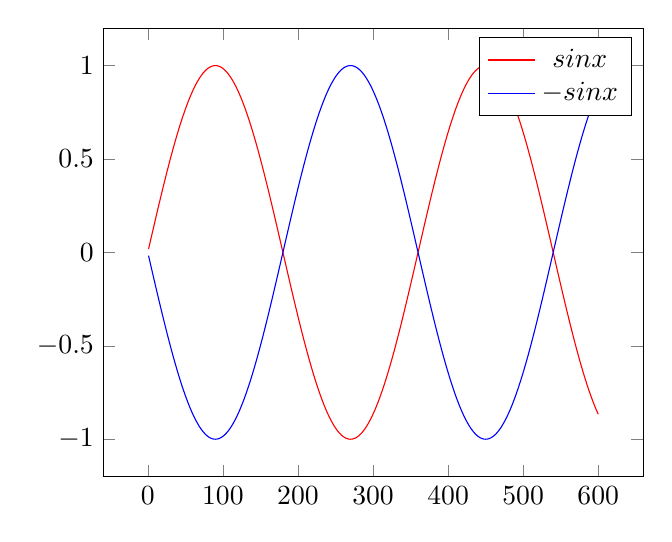
\begin{tikzpicture}
  \begin{axis}[domain=600:1]
    \addplot[samples=500,red] {sin x};
    \addplot[samples=500,blue] {-sin x};
    \legend{$sin x$, $-sin x$}
  \end{axis}
\end{tikzpicture}
\end{center}

However they do not satisfy the first and second conditions, namely that they must be nonnegative both in domain and codomain. A simple $+2$ and domain restriction to both functions can fix this.

But of course neither $\sin x$ nor $-\sin x$ approach $\infty$ as $x\to\infty$ (i.e condition 3). To remedy this we can add $x$, which \textit{does} approach $\infty$ as $x\to\infty$, to both the functions.


We are now left with these two functions, which indeed satisfy all 4 conditions:
\begin{align}
f(x)&=\sin x+x\\
g(x)&=-\sin x+x
\end{align}

Now, to cement this particular example, we'll come up with a strictly increasing sequence of numbers that match condition 4:

$$\left(\frac{(2i+1)\pi}{2}\right)_{i=0}^\infty$$

And it is clear from the properties of the $\sin$ function that this is true.

\section{Problem 3}
\subsection{Part a}
\textbf{Problem:} Give a list $L$ with $6$ distinct elements such that no sublist of size $4$ is strictly increasing and no sublist of size $3$ is strictly decreasing.
\\\\
\textbf{Solution:} After much guesswork I came up with this: $(23,20,26,22,27,24)$. However, since subtraction respects the total ordering of the integers, we can simply pick the smallest entry in the list $k$ and subtract $k-1$ from all entries to arrive at a simpler list. In this case we subtract 19 from each entry:

$$(4,1,7,3,8,5)$$

\subsection{Part b}
\textbf{Problem:} Given two positive integers $s$ and $t$, show how one might construct a list with $st$ distinct elements that has no increasing sublist of size $t+1$ and no decreasing sublist of size $s+1$.
\\\\
\textbf{Solution:} Looking at my simplified answer in part a, it would seem that the list taken by using the even indices is strictly increasing and the same goes for the odd ones. However, as a whole, the list is not increasing. This may be a necessary precondition for a list to satisfy this more general problem.

That said, I have heard of a theorem that guarantees that such a sequence there must be a sublist of $s$ or $t$ that is increasing or decreasing. I don't know how to leverage that to create an actual construction though...

\section{Problem 4}
\subsection{Part a}
\textbf{Problem:} Find all possible partitions of the set $S=\{1,2,3,4\}$
\\\\
\textbf{Solution:} The number of partitions in an $n$ element set is the $n$th bell number denoted $B_n$. That said, I can't be bothered (or trusted) to accurately enumerate all partitions of a 4 element set, so I just made a computer program that does instead. Here is the result: \newline

\textbf{1 Set Case:}
$$\{\{1,2,3,4\}\}$$

\textbf{2 Set Cases:}
\begin{gather*}
\{\{1,2\},\{3,4\}\}\\
\{\{1,3\},\{2,4\}\}\\
\{\{1,4\},\{3,2\}\}\\
\{\{1,2,3\},\{4\}\}\\
\{\{1,2,4\},\{3\}\}\\
\{\{1,3,4\},\{2\}\}\\
\{\{2,3,4\},\{1\}\}
\end{gather*}

\textbf{3 Set Cases:}
\begin{gather*}
\{\{1,2\},\{3\},\{4\}\}\\
\{\{1,3\},\{2\},\{4\}\}\\
\{\{1,4\},\{3\},\{2\}\}\\
\{\{2,3\},\{1\},\{4\}\}\\
\{\{2,4\},\{3\},\{1\}\}\\
\{\{3,4\},\{1\},\{2\}\}
\end{gather*}

\textbf{4 Set Case:}
$$\{\{1\},\{2\},\{3\},\{4\}\}$$

In total there are 1 one set partition, 7 two set partitions, $6$ three set partitions, and 1 four set partition. A total of \textbf{15} partitions of a 4 element set. (note that partitions do not include the empty set $\emptyset$)

\subsection{Part b and c}
Parts b and c refer to 2 conditions of a set of subsets $P$ of a given set $S$:

\textbf{Condition 1:} for every $s\in S$ there exists a $p\in P$ such that $s\in p$.

\textbf{Condition 2:} for every $p_1,p_2\in P$ the following holds: $p_1\not=p_2\rightarrow p_1\cap p_2=\emptyset$

\subsubsection{Part b}
\textbf{Problem:} Give a set of subsets of the set $S=\{1,2,3,4\}$ that fulfills Condition 1 but not 2.
\\\\
\textbf{Solution:} Here's one: $\{\{1,2,3,4\},\{1,2,3\}\}$

\subsubsection{Part c}
\textbf{Problem:} Give a set of subsets of the set $S=\{1,2,3,4\}$ that fulfills Condition 2 but not 1.
\\\\
\textbf{Solution:} Here's one: $\{\{1,2\},\{3\}\}$

\subsection{Part d}
\textbf{Problem:} Give a partition of the set $\{1\}$.
\\\\
\textbf{Solution:} There exists only 1 partition of the above set, namely: $\{\{1\}\}$

\section{Problem 5}
\textbf{Problem:} Give 2 rectangular prisms such that $V_1>V_2$ and $L_1>L_2$ and $S_1<S_2$. Where $V$ is volume, $L$ is the total side length and $S$ is the surface area.
\\\\
\textbf{Solution:} Given that box 1 has sides $a,b,c$ and that box 2 has sides $x,y,z$ we can express this problem as a system of inequalities:

\begin{align*}
V_1>V_2&\equiv abc>xyz\\
L_1>L_2&\equiv 4(a+b+c)>4(x+y+z)\\
S_1<S_2&\equiv 2(ab+bc+ac)>2(xy+yz+xz)
\end{align*}

However notice that the constants can be canceled out on both sides so the system of inequalities becomes:

\begin{gather*}
abc>xyz\\
a+b+c>x+y+z\\
ab+bc+ac>xy+yz+xz
\end{gather*}

From here I could not generate a $6$-tuple of numbers that satisfies the above...

6 degrees of freedom are a lot to brute force by hand or even computationally. That said, I think the answer revolves around the following inequality of two numbers:

$$s+t>st$$

This is generally true (bar some edge cases) when $0<s,t<1$. Leveraging the fact that the product of these number is smaller than their sum is key... I think. With 3 variables we can introduce another quantity leading to something like this:
$$s+t+u>stu>st+tu+su$$
or maybe
$$s+t+u>st+tu+su>stu$$
or even
$$st+tu+su>s+t+u>stu$$

That's all I can come up with.
\end{document}
